\graphicspath{{./figures/}}
\title{}
\date{}
\begin{document}
\begin{frame}
    \titlepage
\end{frame}

\begin{frame}{last time}
    \begin{itemize}
    \item bootstrapping ROP
        \begin{itemize}
        \item look for gadget that sets RSP
        \item use to point to ROP chain
        \end{itemize}
    \item jump-oriented programming
        \begin{itemize}
        \item looking for ``dispatcher gadget'' (incr pointer + jump using it)
        \item form loop returning back to dispatcher gadget
        \end{itemize}
    \item ASLR
        \begin{itemize}
        \item how much randomness; limits with 32-bit systems
        \item keeping executables/libraries together?
        \end{itemize}
    \end{itemize}
\end{frame}

\begin{frame}{scheduling note}
    \begin{itemize}
    \item no class Monday
    \item week's quiz due Wednesday
    \item ROP assignment will be ready by Friday (probably by tomorrow morning)
    \end{itemize}
\end{frame}

\usetikzlibrary{arrows.meta,decorations.pathreplacing,decorations.pathmorphing}
\begin{frame}<1>[fragile,label=aslrTogether]{exes, libraries stay together}
\begin{tikzpicture}[remember picture]
\draw[thick,decorate,decoration={zigzag}] (0, 0) -- (6, 0);
\draw[thick] (0, 0) -- (0, -7);
\draw[thick] (6, 0) -- (6, -7);
\draw[thick,decorate,decoration={zigzag}] (0, -7) -- (6, -7);
\draw[thick,fill=yellow!10] (0, -1) rectangle ++(6, -0.8) node[midway] {foo.exe globals};
\draw[thick,fill=yellow!10] (0, -2) rectangle ++(6, -1.3) node[midway] {foo.exe code};
\draw[thick,fill=yellow!10] (0, -3.5) rectangle ++(6, -0.9) node[midway,align=center] {foo.exe constants \\ (likely has VTables)};
\draw[very thick,Latex-] (6, -4.4) -- ++ (1cm, 0cm) node[right] {this address can be randomized};
\draw[very thick,decorate,decoration={brace,mirror}] (6.1, -4.4) -- ++ (0cm, 3.4) node[midway,right,align=left] {
    must stay together \\
    code uses offset(\%rip) \\
    to access globals, constants
};
\end{tikzpicture}
\end{frame}



\subsection{alternate approach: Windows}

\begin{frame}{relocating: Windows}
    \begin{itemize}
        \item Windows will \myemph{edit code} to relocate
            \begin{itemize}
            \item not everything uses a GOT-like lookup table
            \end{itemize}
        \item typically one fixed location per program/library \textbf{per boot}
            \begin{itemize}
                \item same address used across all instances of program/library
                \item still allows sharing memory
            \end{itemize}
        \item fixup once per program/library per boot
            \begin{itemize}
                \item before ASLR: code could be pre-relocated
            \end{itemize}
        \item Windows + Visual Studio had `full' ASLR by default since 2010
    \end{itemize}
\end{frame}

\begin{frame}{Windows ASLR limitation}
    \begin{itemize}
        \item same address in all programs --- not very useful against local exploits
    \end{itemize}
\end{frame}



\subsection{making ASLR: removing hard-coded addresses}
\begin{frame}{PIC: Linux, OS X}
    \begin{itemize}
        \item Linux, OS X: position-independent code
        \item allows libraries code pages to be shared
        \item \ldots even if loaded at different addresses
        \vspace{.5cm}
        \item avoids per-boot randomization of Windows, but\ldots
    \end{itemize}
\end{frame}


\subsubsection{without absolute}
\begin{frame}[fragile,label=ex]{exercise: avoiding absolute addresses}
\lstset{
    language=myasm,
    style=smaller,
    escapeinside=~~,
}
\begin{tikzpicture}
\node[anchor=north east] (code) at (-1, 0) {
\begin{lstlisting}
foo:
	movl	$3, %eax
	cmpq	$5, %rdi
	ja	defaultCase
	jmp	*lookupTable(,%rdi,8)
returnOne:
        movl    $1, %eax
        ret
returnTwo:
        movl    $2, %eax
defaultCase:
        ret
\end{lstlisting}
};
\node[anchor=north west] (code2) at (-.5, 0) {
\begin{lstlisting}
lookupTable:
    .quad returnOne
    .quad returnTwo
    .quad returnOne
    .quad returnTwo
    .quad returnOne
    .quad returnOne
\end{lstlisting}
};
\end{tikzpicture}
\begin{itemize}
    \item exercise: rewrite this without absolute addresses
    \item but fast
\end{itemize}
\end{frame}



\subsection{changes with position-independent code}


\newcommand{\myemphTwo}[1]{\myemph<2>{#1}}%
\newcommand{\myemphThree}[1]{\myemph<3>{#1}}%
\newcommand{\myemphFour}[1]{\myemph<{#1}}%
\newcommand{\antiEmphThree}[1]{{\color<3>{blue}#1}}%
\newcommand{\antiEmphFour}[1]{{\color<4>{blue}#1}}%
\begin{frame}[fragile,label=PIEjtasm]{PIE jump-table}
\begin{tikzpicture}
\node[anchor=north east] (code) at (-1, 0) {
\lstset{
    language=myasm,
    style=smaller,
    escapeinside=~~,
}
\begin{lstlisting}
foo:
  movl	 $3, %eax
  cmpq	 $5, %rdi
  ja	 retDefault
  leaq	 ~\myemphTwo{jumpTable(\%rip)},~%rax
  movslq ~\myemphTwo{(\%rax,\%rdi,4)},~%rdx
  addq	 %rdx, %rax
  ~\myemphTwo{\bfseries jmp}~   ~\myemphTwo{*\%rax}~
returnTwo:
  movl  $2, %eax
  ret
returnOne:
  movl  $1, %eax
defaultCase:
  ret
\end{lstlisting}
};
\node[anchor=north west] (code2) at ([xshift=2cm]code.north east) {
\lstset{
    language={},
    style=smaller,
    escapeinside=~~,
}
\begin{lstlisting}
  .section	.rodata
jumpTable:
  .long	returnOne-jumpTable
  .long	returnTwo-jumpTable
  .long	returnOne-jumpTable
  .long	returnTwo-jumpTable
  .long	returnOne-jumpTable
  .long	returnOne-jumpTable
\end{lstlisting}
};
\end{tikzpicture}
\end{frame}

\begin{frame}[fragile,label=PIEjt]{PIE jump-table}
\begin{tikzpicture}
\node[anchor=north east] (code) at (-1, 0) {
\lstset{
    language=myasm,
    style=smaller,
    escapeinside=~~,
}
\begin{lstlisting}
~\myemphTwo{00000000000007ab}~ <foo>:
b8 03 00 00 00       	mov    $0x3,%eax
48 83 ff 05             cmp    $0x5,%rdi
77 1b                	ja     7d0 <foo+0x25>
48 8d 05 ab 00 00 00 	lea    ~\myemphThree{0xab(\%rip),}~%rax        # 868
48 63 14 b8          	movslq ~\myemphThree{(\%rax,\%rdi,4),}~%rdx
48 01 d0             	add    %rdx,%rax
ff e0                	jmpq   *%rax
b8 02 00 00 00       	mov    $0x2,%eax
c3                   	retq   
b8 01 00 00 00       	mov    $0x1,%eax
c3                	retq
...
~\textit{\myemphThree{@ 868}}:~ -156 /* offset */
~\textit{\myemphThree{@ 870}}:~ -162
...
\end{lstlisting}
};
\end{tikzpicture}
\end{frame}

\begin{frame}{added cost}
\begin{itemize}
    \item replace \texttt{jmp *jumpTable(,\%rdi,8)}
    \vspace{.5cm}
    \item with:
        \item \texttt{lea} (get table address --- with relative offset)
        \item \texttt{movslq} (do table lookup of offset)
        \item \texttt{add} (add to base)
        \item \texttt{jmp} (to computed base)
\end{itemize}

\end{frame}

\begin{frame}[fragile,label=x86Worse]{32-bit x86 is worse}
    \begin{itemize}
    \item no relative addressing for {\tt mov}, {\tt lea}, \ldots
    \item even changes ``stubs'' for printf:
    \end{itemize}
\lstset{
    language=myasm,
    style=smaller,
    escapeinside=~~,
}
\begin{lstlisting}
// BEFORE: (fixed addresses)
08048310 <__printf_chk@plt>:
 8048310: ff 25 ~\myemphTwo{10 a0 04 08}~  jmp    *0x804a010
    /* 0x804a010 == global offset table entry */

// AFTER: (position-independent)
00000490 <__printf_chk@plt>:
 490:	ff a3 10 00 00 00    jmp    *0x10~\myemphThree{(\%ebx)}~
    /* %ebx --- address of global offset table */
    /* needs to be set by caller */
\end{lstlisting}
\end{frame}



\subsection{PIE}

\begin{frame}{PIE}
    \begin{itemize}
    \item position-independent executables (PIE)
        \begin{itemize}
        \item no hardcoded addresses
        \end{itemize}
    \item alternative: \myemph{edit code (not global offset table) at load time}
        \begin{itemize}
        \item Windows solution
        \end{itemize}
    \item GCC: \texttt{-pie -fPIE}
        \begin{itemize}
        \item \texttt{-pie} is linking option
        \item \texttt{-fPIE} is compilation option
        \item related option: \texttt{-fPIC} (position independent code)
            \begin{itemize}
            \item used to compile runtime-loaded libraries
            \end{itemize}
        \end{itemize}
    \end{itemize}
\end{frame}




\subsection{position-independent cost}

{
\providecommand{\myemphTwo}[1]{\myemph<2>{#1}}%
\providecommand{\myemphThree}[1]{\myemph<3>{#1}}%
\providecommand{\myemphFour}[1]{\myemph<{#1}}%
\providecommand{\antiEmphThree}[1]{{\color<3>{blue}#1}}%
\providecommand{\antiEmphFour}[1]{{\color<4>{blue}#1}}%
\begin{frame}[fragile,label=hardCodedAsm]{hard-coded addresses? (64-bit)}
\lstset{language=C,style=small}
\begin{tikzpicture}
\node[anchor=north east] (code) at (-1, 0) {
\begin{lstlisting}
int foo(long n) {
    switch (n) {
    case 0: 
    case 2:
    case 4:
    case 5:
        return 1;
    case 1:
    case 3:
        return 2;
    default:
        return 3;
    }
}
\end{lstlisting}
};
\draw[thick] (-.75, 0) -- (-.75,-7);
\node[anchor=north west,align=left] (disasm) at (-.5, 0) {
\lstset{
    language=myasm,
    style=smaller,
    escapeinside=~~,
}
\begin{lstlisting}
foo:
	movl	$3, %eax
	cmpq	$5, %rdi
	ja	defaultCase
	jmp	*lookupTable(,%rdi,8)
        /* code for defaultCase, returnOne, returnTwo */
        ...
	.section	.rodata
lookupTable: /* read-only pointers: */
	.quad	returnOne
	.quad	returnTwo
	.quad	returnOne
	.quad	returnTwo
	.quad	returnOne
	.quad	returnOne
\end{lstlisting}
};
\end{tikzpicture}
\end{frame}


\begin{frame}[fragile,label=hardCodedDisasm]{hard-coded addresses? (64-bit)}
\lstset{language=C,style=small}
\begin{tikzpicture}
\node[anchor=north east] (code) at (-1, 0) {
\begin{lstlisting}
int foo(long n) {
    switch (n) {
    case 0: 
    case 2:
    case 4:
    case 5:
        return 1;
    case 1:
    case 3:
        return 2;
    default:
        return 3;
    }
}
\end{lstlisting}
};
\draw[thick] (-.75, 0) -- (-.75,-7);
\node[anchor=north west,align=left] (disasm) at (-.5, 0) {
\lstset{
    language=myasm,
    style=smaller,
    escapeinside=~~,
}
\begin{lstlisting}
~\textit{400570 <foo>}~:
b8 03 00 00 00    mov    $0x3,%eax
48 83 ff 05       cmp    $0x5,%rdi
        /* jump to defaultCase: */
77 ~\antiEmphThree{12}~            ja     ~\antiEmphThree{0x40058d}~
        /* lookup table jump: */
ff 24 fd
~\myemphTwo{18 06 40 00}~      jmpq   *~\myemphTwo{0x400618}(,\%rdi,8)~
...
 /* lookupTable @ 0x400618 */
~\textit{@ 400618:} \myemphTwo{0x400588}~ /* returnOne */
~\textit{@ 400620:} \myemphTwo{0x400582}~ /* returnTwo */
~\textit{@ 400628:} \myemphTwo{0x400588}~
~\textit{@ 400630:} \myemphTwo{0x400582}~
\end{lstlisting}
};
\end{tikzpicture}
\end{frame}

}


\subsubsection{measurements}
\usetikzlibrary{calc}
\begin{frame}{position independence cost (32-bit)}
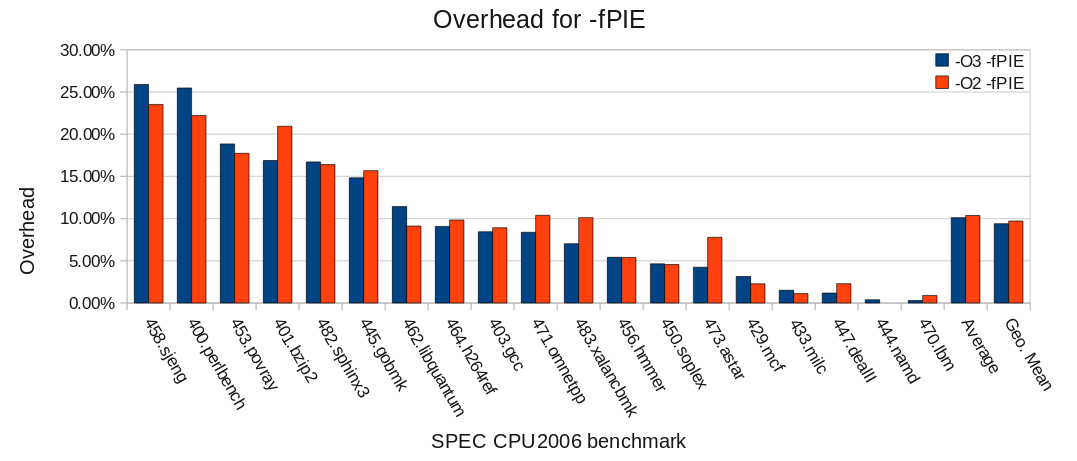
\includegraphics[width=\textwidth]{../mitigate/pie-cost}
\imagecredit{Payer, ``Too much PIE is bad for performance'', ETH Zurich Tech Report}
\end{frame}

\begin{frame}{position independence cost: Linux}
\begin{itemize}
    \item geometric mean of SPECcpu2006 benchmarks on x86 Linux
        \begin{itemize}
            \item with particular version of GCC, etc., etc.
        \end{itemize}
    \item 64-bit: 2-3\% (???)
        \begin{itemize}
        \item ``preliminary result''; couldn't find reliable published data
        \end{itemize}
    \item 32-bit: 9-10\%
    \item depends on compiler, \ldots
\end{itemize}
\end{frame}

\begin{frame}{position independence: deployment}
\begin{itemize}
    \item common for a very long time in dynamic libraries
    \item default for all executables in\ldots
    \vspace{.5cm}
    \item Microsoft Visual Studio 2010 and later
        \begin{itemize}
        \item \texttt{DYNAMICBASE} linker option
        \end{itemize}
    \item OS since 10.7 (2011)
    \item Fedora 23 (2015) and Red Hat Enterprise Linux 8 (2019) and later
        \begin{itemize}
        \item default for ``sensitive'' programs earlier
        \end{itemize}
    \item Ubuntu 16.10 (2016) and later (for 64-bit), 17.10 (2017) and later (for 32-bit)
        \begin{itemize}
        \item default for ``sensitive'' programs earlier
        \end{itemize}
\end{itemize}
\end{frame}



% FIXME: go into example from sudo
\section{sudo exploit example}
\begin{frame}{sudo exploit}
\begin{itemize}
\item this writeup: summary from \url{https://www.openwall.com/lists/oss-security/2021/01/26/3}
\item from group at Qualys
\end{itemize}
\end{frame}

\begin{frame}[fragile,label=sudoBug]{sudo bug}
\begin{itemize}
\item the bug:
\end{itemize}
\begin{lstlisting}[language=C++,style=smaller]
for (size = 0, av = NewArgv + 1; *av; av++)
     size += strlen(*av) + 1;
if (size == 0 || (user_args = malloc(size)) == NULL) { ... }
...
for (to = user_args, av = NewArgv + 1; (from = *av); av++) {
while (*from) {
  if (from[0] == '\\' && !isspace((unsigned char)from[1]))
    from++;
  *to++ = *from++;
...
\end{lstlisting}
\begin{itemize}
\item can skip \texttt{\textbackslash 0} if prefixed with backslash
\item but \texttt{strlen} used to allocate buffer
\item disagreement about copied string length
\item heap overflow!
\end{itemize}
\end{frame}

\begin{frame}{brute-forcing?}
\begin{itemize}
\item method: tried to lots of buffer overflows, get crashes
\item looked at them by hand, found interesting ones\ldots
\end{itemize}
\end{frame}

\begin{frame}[fragile,label=oneCrash]{one crash}
% FIXME: picture showing adjacent struct
\begin{lstlisting}[language={},style=script]
0x000056291a25d502 in process_hooks_getenv (name=name@...ry=0x7f4a6d7dc046 "SYSTEMD_BYPASS_USERDB", value=value@...ry=0x7ffc595cc240) at ../../src/hooks.c:108

=> 0x56291a25d502 <process_hooks_getenv+82>:    callq  *0x8(%rbx)

108         rc = hook->u.getenv_fn(name, &val, hook->closure);
\end{lstlisting}
\begin{itemize}
\item they overwrote a function pointer on the heap!
\item next inquiry: where did that usually point?
\end{itemize}
\end{frame}

\begin{frame}[fragile,label=sudoersSoCode]{sudoers.so}
\begin{lstlisting}[language={},style=smaller]
    *** interesting standard library function: ***
0000000000008a00 <execv@plt>:
    8a00:      endbr64 
    8a04:      bnd jmpq *0x55565(%rip)        # 5df70 <execv@GLIBC_2.2.5>
    8a0b:      nopl   0x0(%rax,%rax,1)
...
    *** usual value of function pointer: ***
000000000000ea00 <sudoers_hook_getenv>:
    ea00:      endbr64 
    ea04:      xor    %eax,%eax
    ea06:      cmpb   $0x0,0x51d36(%rip)        # 60743 <sudoers_policy@@Base+0x2003>
    ea0d:      jne    eaf8 <freeaddrinfo@plt+0x60a8>
    ea13:      cmpq   $0x0,0x51d45(%rip)        # 60760 <sudoers_policy@@Base+0x2020>
\end{lstlisting}
\begin{itemize}
\item<2-> observations (that hold true even with ASLR):
    \begin{itemize}
    \item addr(\texttt{execv@plt}) - addr(\texttt{sudoers\_hook\_getenv}) = \texttt{-0x6000}
    \item last 12 bits of execv@plt always \texttt{a00} (page alignment)
    \end{itemize}
\end{itemize}
\end{frame}

\begin{frame}{changing pointer (part one)}
\begin{itemize}
\item suppose hook\_getenv pointer is \texttt{0xabcdef8a00}
    \begin{itemize}
    \item as bytes: \texttt{\myemph{00 8a} ef cd ab 00 00 00}
    \end{itemize}
\item then execv@plt pointer is \texttt{0xabcdef3a00}
    \begin{itemize}
    \item as bytes: \texttt{\myemph{00 3a} ef cd ab 00 00 00}
    \end{itemize}
\vspace{.5cm}
\item only need to change the last two bytes
\item also: same change would work if pointer had different high bits
\item<2-> only four bits of random data from ASLR!
\end{itemize}
\end{frame}

\begin{frame}{changing pointer (part two)}
\begin{itemize}
\item solution: guess hook\_getenv pointer at  \texttt{0x} (unknown) \texttt{8a00}
\item overwrite last two bytes with \texttt{00 3a}
\vspace{.5cm}
\item if right: will execute your program
\item if wrong: will crash
\vspace{.5cm}
\item<2-> what if crashes? try again! 
    \begin{itemize}
    \item would work about once every 16 tries\ldots
    \item but actual exploit needed to write a 00 byte at the end (strcpy)
    \item so worked `only' about once every 4096 tries
    \end{itemize}
\end{itemize}
\end{frame}

\begin{frame}{into exploit}
\begin{itemize}
\item make \texttt{SYSTEMD\_BYPASS\_USERDB} program in current directory
\item run sudo, triggering buffer overflow to change \\ \texttt{\small sudoers\_hook\_getenv("SYSTEMD\_BYPASS\_USERDB", ...)} \\  into \\
      \texttt{\small execv(SYSTEMD\_BYPASS\_USERDB, ...)} 
    \begin{itemize}
    \item (well, try to change --- it won't always work)
    \end{itemize}
\end{itemize}
\end{frame}



\section{heap smashing}

\begin{frame}{heap smashing}
    \begin{itemize}
    \item ``lucky'' adjancent objects
    \item same things possible on stack
    \item but stack overflows had nice generic ``stack smashing''
    \item is there an equivalent for the heap?
    \item yes (mostly)
    \end{itemize}
\end{frame}




\subsection{heap bookkeeping}

\tikzset{
    stackBox/.style={very thick},
    onStack/.style={thick},
    frameOne/.style={fill=blue!15},
    frameTwo/.style={fill=red!15},
    markLine/.style={blue!50!black},
    markLineB/.style={red!90!black},
    hiLine/.style={red!90!black},
}

\begin{frame}{diversion: implementing malloc/new}
    \begin{itemize}
    \item many ways to implement malloc/new
    \item we will talk about one common technique
    \end{itemize}
\end{frame}

\begin{frame}[fragile,label=heapLayout]{heap object}
\begin{tikzpicture}
\node[anchor=north east] (code) at (-1,0) {
\begin{lstlisting}
struct AllocInfo {
  bool free;
  int size;
  AllocInfo *prev;
  AllocInfo *next;
};
\end{lstlisting}
};

\tikzset{xscale=0.9}
\begin{scope}[overlay]
    \draw[stackBox,fill=black!20] (0, 1) rectangle (3, -7);

    \draw[onStack] (0, 1) rectangle (3, 0) node[midway,font=\small,align=center] {free space \\ (deleted obj.)};
    \draw[onStack,fill=white] (0, -0.0) rectangle (3, -0.5) node[midway,font=\small] (freeANext) {next};
    \draw[onStack,fill=white] (0, -0.5) rectangle (3, -1.0) node[midway,font=\small] (freeAPrev) {prev};
    \draw[onStack,fill=white] (0, -1.0) rectangle (3, -1.5) node[midway,font=\small] (freeASize) {size/free};

    \draw[very thick, red, rounded corners] (0, 1) rectangle (3, -1.5);

    \draw[onStack,fill=blue!20] (0, -1.5) rectangle (3, -3.0) node[midway,font=\small,align=center] (freeBAlloc) {new'd object};
    \draw[onStack,fill=white] (0, -3.0) rectangle (3, -3.5) node[midway,font=\small] (freeBSize) {size/free};
    
    \draw[very thick, red, rounded corners] (0, -1.5) rectangle (3, -3.5);

    \draw[onStack] (0, -3.5) rectangle (3, -5.0) node[midway,font=\small] {free space};
    \draw[onStack,fill=white] (0, -5.0) rectangle (3, -5.5) node[midway,font=\small] (freeCNext) {next};
    \draw[onStack,fill=white] (0, -5.5) rectangle (3, -6.0) node[midway,font=\small] (freeCPrev) {prev};
    \draw[onStack,fill=white] (0, -6.0) rectangle (3, -6.5) node[midway,font=\small] (freeCSize) {size/free};
    
    \draw[very thick, red, rounded corners] (0, -3.5) rectangle (3, -6.5);
    
    \draw[-Latex,blue,thick] (freeAPrev) -- ++(1.75cm,0cm) |- (freeCSize);
    \draw[-Latex,blue,thick] (freeCNext) -- ++(2.00cm,0cm) |- (freeASize);
    \draw[-Latex,blue,thick,opacity=0.5] (freeCPrev) -- ++(1.25cm,0cm) -- ++(0cm,-2cm);
    \draw[-Latex,blue,thick,opacity=0.5] (freeANext) -- ++(1.75cm,0cm) -- ++(0cm,2cm);
\end{scope}
\draw[-Latex,line width=3pt,black!50] (3.5,-2.25) -- (5.5,-2.25) node[black,midway,above,font=\small\tt] {free};
\begin{scope}[overlay,xshift=6cm,name prefix=sec-]
    \draw[stackBox,fill=black!20] (0, 1) rectangle (3, -7);

    \draw[onStack] (0, 1) rectangle (3, -5.0) node[midway,font=\small] {free space};
    \draw[onStack,fill=white] (0, -5.0) rectangle (3, -5.5) node[midway,font=\small] (freeCNext) {next};
    \draw[onStack,fill=white] (0, -5.5) rectangle (3, -6.0) node[midway,font=\small] (freeCPrev) {prev};
    \draw[onStack,fill=white] (0, -6.0) rectangle (3, -6.5) node[midway,font=\small] (freeCSize) {size/free};
    
    \draw[-Latex,blue,thick,opacity=0.5] (freeCPrev) -- ++(1.25cm,0cm) -- ++(0cm,-2cm);
    \draw[-Latex,blue,thick,opacity=0.5] (freeCNext) -- ++(1.75cm,0cm) -- ++(0cm,2cm);
\end{scope}
\end{tikzpicture}
\end{frame}

\begin{frame}[fragile,label=freeImpl]{implementing free()}
\lstset{
    style=small,
    language=C,
    moredelim={**[is][\btHL<2|handout:0>]{~2~}{~end~}},
}
\begin{lstlisting}
int free(void *object) {
    ...
    block_after = object + object_size;
    if (block_after->free) {
        /* unlink from list, about to merge with previous block */
        new_block->size += block_after->size;
        ~2~block_after->prev->next = block_after->next;~end~
        block_after->next->prev = block_after->prev;
    }
    ...
}
\end{lstlisting}
\begin{itemize}
\item<2> \large \myemph<2>{arbitrary memory write}
\end{itemize}
\end{frame}



\subsection{bookkeeping to pointer subterfuge}
\usetikzlibrary{arrows.meta,decorations.pathreplacing,patterns}

\tikzset{
    stackBox/.style={very thick},
    onStack/.style={thick},
}
\begin{frame}[fragile,label=vulnHeapSmash]{vulnerable code}
\lstset{
    style=small,
    language=C,
    moredelim={**[is][\btHL<4|handout:0>]{~2~}{~end~}},
    moredelim={**[is][\btHL<2-3|handout:0>]{~3~}{~end~}},
    moredelim={**[is][\btHL<6-|handout:0>]{~6~}{~end~}},
}
\begin{tikzpicture}
\node[anchor=north east] (code) at (-1,0) {
\begin{lstlisting}
char *buffer = malloc(100);
... 
~2~strcpy(buffer, attacker_supplied);~end~
... 
~3~free(buffer);~end~
~6~free(other_thing);~end~
...
\end{lstlisting}
};

\tikzset{xscale=0.9}
\begin{scope}[overlay]
    \draw[stackBox,fill=black!20] (0, 1) rectangle (3, -7);

    \begin{pgfonlayer}{fg}
    \draw[very thick, orange, rounded corners] (0, 1) rectangle (3, -1.5);
    \draw[very thick, orange, rounded corners] (0, -1.5) rectangle (3, -3.5);
    \draw[very thick, orange, rounded corners] (0, -3.5) rectangle (3, -6.5);
    \draw[very thick,-Latex] (3.1, -6.5) -- ++(0, 3) node[sloped,right] {incr. addrs};
    \end{pgfonlayer}

    \draw[onStack] (0, 1) rectangle (3, 0) node[midway,font=\small] {free space};
    \draw[onStack,fill=white] (0, -0.0) rectangle (3, -0.5) node[midway,font=\small] (freeANext) {next};
    \draw[onStack,fill=white] (0, -0.5) rectangle (3, -1.0) node[midway,font=\small] (freeAPrev) {prev};
    \draw[onStack,fill=white] (0, -1.0) rectangle (3, -1.5) node[midway,font=\small] (freeASize) {size/free};

    \draw[onStack,fill=blue!20] (0, -1.7) rectangle (3, -3.0) node[midway,font=\small,align=center] (freeBAlloc) {alloc'd object};
    \begin{visibleenv}<4->
    \fill[pattern color=red,pattern=north west lines] (0, -0.0) rectangle (3, -3.0);
    \end{visibleenv}
    \draw[onStack,fill=white] (0, -3.0) rectangle (3, -3.5) node[midway,font=\small] (freeBSize) {size/free};

    \draw[onStack] (0, -3.5) rectangle (3, -5.0) node[midway,font=\small] {free space};
    \draw[onStack,fill=white] (0, -5.0) rectangle (3, -5.5) node[midway,font=\small] (freeCNext) {next};
    \draw[onStack,fill=white] (0, -5.5) rectangle (3, -6.0) node[midway,font=\small] (freeCPrev) {prev};
    \draw[onStack,fill=white] (0, -6.0) rectangle (3, -6.5) node[midway,font=\small] (freeCSize) {size/free};
    
    \draw[-Latex,blue,thick] (freeAPrev) -- ++(1.75cm,0cm) -- ++ (0cm, -1cm) -- ++ (4cm,0cm); %|- (freeCSize);
    \draw[-Latex,blue,thick] (freeCNext) -- ++(2.00cm,0cm) -- ++ (0cm, 1cm) -- ++ (4cm,0cm); % |- (freeASize);
    \draw[-Latex,blue,thick,opacity=0.5] (freeCPrev) -- ++(1.25cm,0cm) -- ++(0cm,-2cm);
    \draw[-Latex,blue,thick,opacity=0.5] (freeANext) -- ++(1.75cm,0cm) -- ++(0cm,2cm);

    \begin{visibleenv}<4->
        \begin{scope}[xshift=-5cm,yshift=-3cm]
        \tikzset{gotBox/.style={thick,fill=orange!30}}
        \draw[gotBox,alt=<6>{fill=red!10}] (0, -1) rectangle (4, -1.5) node[midway,font=\small] (freeEntry) {GOT entry: free};
        \draw[gotBox] (0, -1.5) rectangle (4, -2) node[midway,font=\small] {GOT entry: malloc };
        \draw[gotBox] (0, -2) rectangle (4, -2.5) node[midway,font=\small] (printfEntry) {GOT entry: printf };
        \draw[gotBox] (0, -2.5) rectangle (4, -3.0) node[midway,font=\small] (gotFopen) {GOT entry: fopen };
        \end{scope}
        \draw[-Latex,red,ultra thick,dashed] (freeAPrev) -- ++(-2cm,0cm) |- ([yshift=-.25cm]printfEntry.east);
        \draw[-Latex,red,ultra thick,dashed] (freeANext) -- ++(-2.5cm,0cm) -- ++(0cm,-2.5cm) -- ++(-.5cm,0cm) node [black,solid,draw,left,align=left,fill=white] (scode) {shellcode/etc.};
    \end{visibleenv}
    \begin{visibleenv}<3>
        \draw[ultra thick,decorate,decoration={brace}] (3.15, 1) -- ++ (0, -2.5) node[midway,right,font=\small,align=left] {to be removed \\ from linked list};
    \end{visibleenv}
    \begin{visibleenv}<2>
        \draw[ultra thick,decorate,decoration={brace}] (3.15, 1) -- ++ (0, -5.5) node[midway,right,font=\small,align=left] {free() tries \\ to merge these};
    \end{visibleenv}
    \begin{visibleenv}<5->
        \begin{scope}[xshift=-5cm,yshift=-3cm]
        \draw[blue,opacity=0.8] (-3, -2) rectangle (0, -2.5) node[midway,font=\small] {prev->size/free};
        \draw[blue,opacity=0.8] (-3, -1.5) rectangle (0, -2) node[midway,font=\small] {prev->prev};
        \draw[blue,opacity=0.8] (-3, -1) rectangle (0, -1.5) node[midway,font=\small] {prev->next};
        \end{scope}
        \draw[-Latex,blue,ultra thick,dotted] (freeEntry.north) -- ++(0cm,.1cm) -| (scode.south);
        \node[draw,very thick] at ([xshift=0cm,yshift=-1.5cm]gotFopen.south west) {
            \lstinline|block_after->prev->next = block_after->next|
        };
    \end{visibleenv}
\end{scope}
\end{tikzpicture}
\end{frame}




% FIXME: exercise, using linked-list heap exploit to write something
\subsection{exericse}
\usetikzlibrary{arrows.meta,matrix,fit}
\begin{frame}[fragile,label=heapSubterExercise]{heap overflow exercise}
\begin{lstlisting}[language=C++,style=script]
void operator delete(void *p) {
    ...
    block_after->prev->next = block_after->next;
    ...
}
...
class MyBuffer : public GenericMyBuffer {
public:
    virtual void store(const char *p) override {
        strcpy(buffer, p);
    }
private:
    char buffer[64];
};
...
    GenericMyBuffer *a = new MyBuffer;
    ...
    a->store(attacker_controlled);
    ...
    delete a;
    ...
\end{lstlisting}
\begin{tikzpicture}[overlay,remember picture]
\coordinate (place) at ([yshift=-1.5cm,xshift=-1cm]current page.north east);
\matrix[tight matrix,nodes={text width=3cm,font=\fontsize{9}{10}\selectfont,thick},thick,anchor=north east,label={north:heap object layout}]  (diag) at (place) {
    |[draw=none,align=center,font=\it]| when free \& |[draw=none,align=center]| when used \\
    |[fill=yellow!10]| size+free (8 B) \& |[fill=yellow!10,alias=arrowSide]| size+free (8 B) \\
    |[fill=blue!10]| next pointer (8 B) \& |[fill=violet!10]| vtable pointer (8 B) \\
    |[fill=blue!10]| prev pointer (8 B) \& |[alias=bufPt1]| ~ \\
    |[alias=unusedPt1]| ~                  \& |[alias=bufPt2]| ~ \\
    |[alias=unusedPt2]| ~                  \& |[alias=bufPt3]| ~ \\
    |[alias=unusedPt3]| ~                  \& |[fill=green!10]| unused space (16 B) \\
    |[alias=unusedPt4]| \& (next size+free)   \\
     (next size+free) \\
};
\draw[very thick,-Latex] ([xshift=.25cm]arrowSide.north east) -- ++(0cm, -1cm);
\node[inner sep=0mm,fill=violet!10,fit=(bufPt1) (bufPt2) (bufPt3),font=\small,draw,thick] {buffer (64B)};
\node[inner sep=0mm,fill=green!10,fit=(unusedPt1) (unusedPt2) (unusedPt3) (unusedPt4),font=\small,draw,thick] {unused space \\ (?? B)};
\begin{visibleenv}<1>
\node[anchor=north west,align=left,draw,very thick,font=\fontsize{12}{13}\selectfont] at ([xshift=-1cm]diag.south west) {
    exercise 1: \\
    to attack this buffer overflow \\
    by overwriting the heap data structures \\
    does it matter if space after \texttt{a} \\
    is already free or not?
};
\end{visibleenv}
\begin{visibleenv}<2>
\node[anchor=north west,align=left,draw,very thick,font=\fontsize{12}{13}\selectfont] at ([xshift=-1cm]diag.south west) {
    exercise 2:
    if \texttt{a} at address 0x10000, \\ 
    and attacker wants to overwrite \\
    value at address 0x20000 with 0x30000, \\
    where should attacker put 0x20000, 0x30000\\
    in \texttt{attacker\_controlled}? \\

};
\end{visibleenv}
\end{tikzpicture}
\end{frame}


\section{alternate malloc designs?}
\begin{frame}{other malloc designs?}
\begin{itemize}
\item there are a lot of different malloc/new implementations
\item often multiple free lists
\item free block list might not be kept with linked list
\vspace{.5cm}
\item some place metadata next to allocations like this
\item some keep it separate
\vspace{.5cm}
\item usually performance determines which is chosen
\end{itemize}
\end{frame}


\section{use-after-free}

\tikzset{
    stackBox/.style={very thick},
    onStack/.style={thick},
}
\begin{frame}[fragile,label=vulnUAF]{vulnerable code}
\lstset{
    language=C++,
    style=smaller,
    moredelim={**[is][\btHL<2|handout:0>]{~2~}{~end~}},
}
\begin{tikzpicture}
\node[anchor=north east] (code) at (-1,0) {
\begin{lstlisting}
class Foo {
    ...
};
Foo *the_foo;
the_foo = new Foo;
...
delete the_foo;
...
something_else = new Bar(...);
the_foo->something();
\end{lstlisting}
};
\node[draw,anchor=north west,align=left] at (-3,0) {
    {\tt something\_else} likely where {\tt the\_foo} was
};
\begin{visibleenv}<2>
\draw[stackBox] (0, -2) rectangle (3, -5);
\draw[stackBox] (4, -2) rectangle (7, -5);
\draw[onStack,fill=blue!20] (0, -2) rectangle (3, -3) node[midway,align=center,font=\small] { vtable ptr (Foo) };
\draw[onStack,fill=blue!20] (0, -3) rectangle (3, -5) node[midway,align=center,font=\small] {data for Foo };
\draw[onStack,fill=yellow!20] (4, -2) rectangle (7, -3) node[midway,align=center,font=\small] { vtable ptr (Bar)? \\
                                                                                   other data? };
\draw[onStack,fill=yellow!20] (4, -3) rectangle (7, -5) node[midway,align=center,font=\small] { data for Bar  };
\end{visibleenv}
\end{tikzpicture}
\end{frame}



\subsection{pattern}

\begin{frame}{exploiting use after-free}
\begin{itemize}
\item trigger many ``bogus'' frees; then
\item allocate many things of same size with ``right'' pattern  
    \begin{itemize}
    \item pointers to shellcode?
    \item pointers to pointers to {\tt system()}?
    \item objects with something useful in VTable entry?
    \end{itemize}
\item trigger use-after-free thing
\end{itemize}
\end{frame}


\section{backup slides}
\begin{frame}{backup slides}
\end{frame}
\subsection{exercise: using a leak}
\begin{frame}[fragile,label=useLeak1]{exericse: using a leak (1)}
\begin{lstlisting}[language=C++,style=small]
class Foo {
    virtual const char *bar() { ... }
};
...
Foo *f = new Foo;
printf("%s\n", f);
\end{lstlisting}
\begin{itemize}
\item Part 1: What address is most likely leaked by the above?
    \begin{itemize}
    \item A. the location of the Foo object allocated on the heap
    \item B. the location of the first entry in Foo's VTable"
    \item C. the location of the first instruction of Foo::Foo() (Foo's compiler-generated constructor)"
    \item D. the location of the stack pointer
    \end{itemize}
\end{itemize}
\end{frame}


\begin{frame}[fragile,label=useLeak2]{exercise: using a leak (2)}
\begin{lstlisting}[language=C++,style=script]
class Foo {
    virtual const char *bar() { ... }
};
...
Foo *f = new Foo;
char *p = new char[1024];
printf("%s\n", f);
\end{lstlisting}
\begin{itemize}
\item if leaked value was 0x822003 and in a debugger (with \textbf{different randomization}):
    \begin{itemize}
    \item stack pointer was 0x7ffff000
    \item Foo::bar's address was 0x400000
    \item f's address was 0x900000
    \item f's Vtable's address was 0x403000
    \item a ``gadget'' address from the main executable was 0x401034
    \item a ``gadget'' address from the C library was 0x2aaaa40034
    \item p's address was 0x901000
    \end{itemize}
\item which of the above can I compute based on the leak?
\end{itemize}
\end{frame}


\subsection{exercise: using function pointer overwrite}
\begin{frame}[fragile,label=useFPtrOverwrite1]{using function pointer overwrite (1)}
\begin{lstlisting}[language=C,style=script]
struct Example {
    char input[1000];
    void (*process_function)(Example *, long, char *);
};
void vulnerable(struct Example *e) {
    long index;
    char name[1000];
    gets(e->input); /* can overwrite process_function */
    scanf("%ld,%s", &index, &name[0]); /* expects <decimal number>,<string> */
    (e->process_function)(e /* rdi */, index /* rsi */, name /* rdx */);
}
\end{lstlisting}
\begin{itemize}
\item if we overwrite process\_function's address with the address of the gadget
    \texttt{mov \%rsi, \%rsp; ret}, then the beginning of the input
    should contain\ldots \\
    \begin{itemize}
    \item A. the shellcode to run
    \item B. an ROP chain to run
    \item C. the address of shellcode (or existing function) in decimal
    \item D. the address of the ROP chain to run written out in decimal
    \item E. the address of a RET instruction written out in decimal
    \end{itemize}
\end{itemize}
\end{frame}

\iftoggle{heldback}{\excludecomment{soln}}{\includecomment{soln}}
\begin{soln}
\begin{frame}[fragile,label=useFPtrOverwrite1Explain]{explanation}
\begin{lstlisting}[language=C++,style=script]
gets(e->input); /* can overwrite process_function */
scanf("%ld,%s", &index, &name[0]); /* expects <decimal number>,<string> */
(e->process_function)(e /* rdi */, index /* rsi */, name /* rdx */);
\end{lstlisting}
\texttt{"1234,FOO......."} + addr of \texttt{mov \%rsi, \%rsp, ret}
\begin{itemize}
\item arguments setup registers for gadget:
\begin{itemize}
    \item \%rdi (irrelevant) is "1234,FOO..." (copy in e)
    \item \%rsi is 1234 (from scanf)
    \item \%rdx (irrelevant) is "FOO..." (pointer to name)
\end{itemize}
\item mov in gadget: \%rsi (1234) becomes \%rsp
\item ret in gadget: read pointer at 1234, set \%rsp to 1234 + 8
    \begin{itemize}
    \item jump to next gadget (whose address should be stored at 1234)
    \item if that gadget returns, will read new return address from 1238
    \end{itemize}
\end{itemize}
\end{frame}
\end{soln}

\begin{frame}[fragile,label=useFPtrOverwrite2]{using function pointer overwrite (2)}
\begin{lstlisting}[language=C,style=script]
struct Example {
    char input[1000];
    void (*process_function)(Example *, long, char *);
};
void vulnerable(struct Example *e) {
    long index;
    char name[1000];
    gets(e->input); /* can overwrite process_function */
    scanf("%ld,%s", &index, &name[0]); /* expects <decimal number>,<string> */
    (e->process_function)(e /* rdi */, index /* rsi */, name /* rdx */);
}
\end{lstlisting}
\begin{itemize}
\item if we overwrite process\_function's address with the address of the gadget
    \texttt{push \%rdx; jmp *(\%rdi)}, then the beginning of the input should contain\ldots \\
    \begin{itemize}
    \item A. the shellcode to run
    \item B. an ROP chain to run
    \item C. the address of shellcode (or existing function) 
    \item D. the address of the ROP chain 
    \item E. the address of a RET instruction
    \end{itemize}
\end{itemize}
\end{frame}

\begin{soln}
\begin{frame}[fragile,label=useFPtrOverwrite1Explain]{explanation (one option)}
\begin{lstlisting}[language=C++,style=script]
gets(e->input); /* can overwrite process_function */
scanf("%ld,%s", &index, &name[0]); /* expects <decimal number>,<string> */
(e->process_function)(e /* rdi */, index /* rsi */, name /* rdx */);
\end{lstlisting}
\texttt{"FOOBARBAZ......."} + addr of \texttt{push \%rdx; jmp *(\%rdi)}
\begin{itemize}
\item arguments setup registers for gadget:
\begin{itemize}
    \item \%rdi is "FOOBARBAZ...." (copy in e)
    \item \%rsi (irrelevant) is uninitialized? (scanf failed)
    \item \%rdx (irrelevant) is uninitialized? (scanf failed)
\end{itemize}
\item push in gadget: top of stack becomes copy of uninit. value 
\item jmp in gadget
    \begin{itemize}
    \item interpret ``FOOBARBA'' as 8-byte address
    \item jump to that address
    \end{itemize}
\end{itemize}
\end{frame}

\begin{frame}[fragile,label=useFPtrOverwrite2Explain]{explanation (unlikely alternative?)}
\begin{lstlisting}[language=C++,style=script]
gets(e->input); /* can overwrite process_function */
scanf("%ld,%s", &index, &name[0]); /* expects <decimal number>,<string> */
(e->process_function)(e /* rdi */, index /* rsi */, name /* rdx */);
\end{lstlisting}
\texttt{"1234567890,FOO......."} + addr of \texttt{push \%rdx; jmp *(\%rdi)}
\begin{itemize}
\item arguments setup registers for gadget:
\begin{itemize}
    \item \%rdi is address of string "12345678,FOO..." (copy in e)
    \item \%rsi is 12345678
    \item \%rdx is address of string "FOO..." (copy in name)
\end{itemize}
\item push in gadget: top of stack becomes address of "FOO..."
\item jmp in gadget
    \begin{itemize}
    \item interpret \textit{ASCII encoding of ``12345678''} (???) as 8-byte address
    \item jump to that address
    \end{itemize}
\end{itemize}
\end{frame}
\end{soln}


\end{document}
